\documentclass{article}
\usepackage{amsmath}
\usepackage{graphicx}
\usepackage{amsfonts}
\usepackage{amssymb}
\usepackage{bm}
\usepackage[colorlinks=true, linkcolor=black, urlcolor=blue]{hyperref}
\usepackage{fontspec}
\setmainfont{Times New Roman}
\usepackage{listings}
\usepackage{xcolor}
\usepackage{mathtools}
\usepackage[most]{tcolorbox}
\tcbuselibrary{breakable}
\usepackage{fancyvrb}
\usepackage{placeins}
\usepackage{booktabs}
\usepackage{float}
\usepackage[a4paper, margin=1in]{geometry}
\usepackage{subcaption}
\usepackage{tikz}
\usetikzlibrary{arrows.meta,positioning,fit,backgrounds,calc}
\usepackage{pgfplots}
\pgfplotsset{compat=1.18}
\usepackage{float}
% ---------- COLORS ----------
\definecolor{inputblue}{RGB}{66,165,245}
\definecolor{sigmoidpurple}{RGB}{171,71,188}
\definecolor{hidden1}{RGB}{129,199,132}
\definecolor{hidden2}{RGB}{255,193,7}
\definecolor{reluorange}{RGB}{255,167,38}
\definecolor{bncyan}{RGB}{0,188,212}
\definecolor{outputred}{RGB}{244,67,54}
\definecolor{residualgray}{RGB}{96,125,139}

\definecolor{darkblue}{RGB}{35,55,120}
\definecolor{mygreen}{RGB}{0,128,0}
\definecolor{myred}{RGB}{200,50,50}
\definecolor{mypurple}{RGB}{150,0,150}
\definecolor{mygray}{gray}{0.95}

\definecolor{HeaderBlue}{RGB}{35,55,120}
% ---------- TIKZ STYLES ----------
\tikzset{
	>=Latex,
	neuron/.style={
		circle,
		draw,
		thick,
		minimum size=7mm,
		inner sep=0pt
	},
	layerbox/.style={
		draw,
		rounded corners,
		thick,
		inner sep=4pt,
		fill opacity=0.06
	},
	conn/.style={
		-{Latex[length=2mm,width=1.6mm]},
		line width=0.6pt
	}
}


\lstset{
  language=Matlab,
  basicstyle=\small\ttfamily,
  keywordstyle=\color{blue},
  commentstyle=\color{green!70!black},
  stringstyle=\color{red},
  showstringspaces=false,
  frame=single,
  captionpos=b,
  % --- ADD THESE THREE LINES TO FIX LINE BREAKING ---
  breaklines=true,                 % 1. Enables automatic line breaking
  breakatwhitespace=false,         % 2. Allows breaking lines at non-whitespace
  postbreak=\mbox{\textcolor{red}{$\hookrightarrow$}\space} % 3. Adds an arrow to show a line break
}

\begin{document}
\begin{titlepage}
  \centering
  
\includegraphics[width=0.3\textwidth]{download.png} \\[1.5cm]
  {\huge \textbf{K.N. Toosi University}}\\[2cm]
  {\Large \textbf{Aidin Sahneh}}\\[0.5cm] 
  {\large \textbf{\\ Student ID:} 40120243}\\[0.7cm]
  {\Large \textbf{Mani Vafapour}}\\[0.5cm] 
  {\large \textbf{\\ Student ID:} 40123783}\\[0.7cm]
  {\Large \textbf{Hamed Behrouzi Moghaddam}}\\[0.5cm] 
  {\large \textbf{\\ Student ID:} 40215633}\\[0.7cm]
  {\Large \textbf{\\ Course:} Introduction to MachineLearning}\\[0.3cm]
  {\large \textbf{Instructor:} Dr. Nikoofard }\\[0.5cm]
  
  \vspace{1cm}
  % ---------- Colab Link ----------
  {\large \textbf{Question 3 Implementation:}}\\[0.2cm]
  \href{https://colab.research.google.com/drive/1aQ7MT61A5mfuG07QamgAo0H6rMNu7ZfP#scrollTo=5BBY5iAPpW32}{\textbf{\textcolor{blue}{View Google Colab Notebook}}}
  
\end{titlepage}

\newpage
\tableofcontents
\newpage

\section{Question 1: Analysis and Implementation of Masked Convolutional Layer}

\subsection{Mathematical Derivation of Gradients}
In this problem, we define a custom convolutional layer where the effective filter $\tilde{W}$ is computed as the element-wise (Hadamard) product of a weight matrix $W$ and a learnable mask matrix $M$:
\[ \tilde{W} = W \odot M \]
where $W, M \in \mathbb{R}^{K \times K}$. During the backpropagation phase, the gradients of the loss function $L$ with respect to $W$ and $M$ must be derived to update the parameters.

\subsubsection*{Gradient with respect to Weight $W$}
Applying the chain rule, the gradient of the loss $L$ with respect to the weights $W$ is given by:
\[ \frac{\partial L}{\partial W} = \frac{\partial L}{\partial \tilde{W}} \odot \frac{\partial \tilde{W}}{\partial W} \]
Since $\tilde{W}_{i,j} = W_{i,j} \cdot M_{i,j}$, the partial derivative $\frac{\partial \tilde{W}_{i,j}}{\partial W_{i,j}}$ is simply $M_{i,j}$. Therefore, the final gradient is:
\begin{equation}
\frac{\partial L}{\partial W} = \frac{\partial L}{\partial \tilde{W}} \odot M
\end{equation}

\subsubsection*{Gradient with respect to Mask $M$}
Similarly, the gradient with respect to the mask matrix $M$ is:
\[ \frac{\partial L}{\partial M} = \frac{\partial L}{\partial \tilde{W}} \odot \frac{\partial \tilde{W}}{\partial M} \]
Given that $\frac{\partial \tilde{W}_{i,j}}{\partial M_{i,j}} = W_{i,j}$, we obtain:
\begin{equation}
\frac{\partial L}{\partial M} = \frac{\partial L}{\partial \tilde{W}} \odot W
\end{equation}

\newpage
\subsection{Implementation Details in PyTorch}
The implementation utilizes the \texttt{torch.nn.functional.unfold} method to perform the convolution manually. This approach transforms the spatial input into a matrix of sliding blocks (im2col), allowing the convolution operation to be executed via matrix multiplication.




\begin{tcolorbox}[colback=yellow!10!white, colframe=yellow!70!black, title=PyTorch Implementation, fonttitle=\bfseries]
	\begin{lstlisting}[language=Python, basicstyle=\small\ttfamily, breaklines=true]
	import torch
	import torch.nn as nn
	import torch.nn.functional as F
	
	class MaskedConvLayer(nn.Module):
	def __init__(self, kernel_size):
	super(MaskedConvLayer, self).__init__()
	self.kernel_size = kernel_size
	# Learnable parameters
	self.W = nn.Parameter(torch.randn(1, 1, kernel_size, kernel_size))
	self.M = nn.Parameter(torch.randn(1, 1, kernel_size, kernel_size))
	
	def forward(self, x):
	# Hadamard product
	effective_weight = self.W * self.M
	
	# im2col using Unfold
	x_unfold = F.unfold(x, kernel_size=self.kernel_size)
	weight_flat = effective_weight.view(1, -1)
	
	# Matrix multiplication
	out_unfold = weight_flat @ x_unfold
	
	# Reshape to output dimensions
	out_size = x.size(-1) - self.kernel_size + 1
	return out_unfold.view(x.size(0), 1, out_size, out_size)
	\end{lstlisting}
\end{tcolorbox}

\subsection{Verification of Results}
The model was tested with a $1 \times 1 \times 5 \times 5$ input and a $3 \times 3$ kernel using Mean Squared Error (MSE) loss. The numerical outputs obtained after one backward pass are:

\begin{itemize}
	\item \textbf{Initial Loss:} 4.6200
	\item \textbf{Gradient of $W$ (first 3 elements):} $[ 1.1261, -1.0485, 0.1057 ]$
	\item \textbf{Gradient of $M$ (first 3 elements):} $[ 0.4340, -0.3002, -1.0274 ]$
\end{itemize}

The discrepancy between the gradients of $W$ and $M$ confirms that the backpropagation through the element-wise multiplication is working correctly, as each gradient is appropriately scaled by the corresponding value of the other parameter.



\newpage
\section{Question 2: ResNet Bottleneck Architecture and Resource Management}

\subsection{Analytical Calculation of Parameters}
The ResNet Bottleneck block consists of three sequential convolutional layers. Given an input with $C_{in}=256$, the architecture uses a $1 \times 1$ reduction layer, a $3 \times 3$ spatial processing layer, and a $1 \times 1$ expansion layer. The number of parameters for each layer (excluding bias and Batch Normalization) is calculated using the formula: $\text{Params} = K \times K \times C_{in} \times C_{out}$.

\subsubsection*{Standard Configuration (64 Middle Filters)}
\begin{itemize}
	\item \textbf{Layer 1 ($1 \times 1, 64$ filters):} $1 \times 1 \times 256 \times 64 = 16,384$
	\item \textbf{Layer 2 ($3 \times 3, 64$ filters):} $3 \times 3 \times 64 \times 64 = 36,864$
	\item \textbf{Layer 3 ($1 \times 1, 256$ filters):} $1 \times 1 \times 64 \times 256 = 16,384$
\end{itemize}
\textbf{Total Parameters:} $16,384 + 36,864 + 16,384 = \mathbf{69,632}$.

\subsection*{Impact of Reducing Middle Filters to 32}
To optimize the model for edge devices with severe memory constraints, we reduce the middle filters ($C_{mid}$) from 64 to 32.

\subsubsection*{Parameter Reduction Analysis}
The new parameter count is calculated as follows:
\begin{itemize}
	\item \textbf{Layer 1:} $1 \times 1 \times 256 \times 32 = 8,192$
	\item \textbf{Layer 2:} $3 \times 3 \times 32 \times 32 = 9,216$
	\item \textbf{Layer 3:} $1 \times 1 \times 32 \times 256 = 8,192$
\end{itemize}
\textbf{New Total:} $25,600$. 
The \textbf{percentage reduction} is:
\[ \frac{69,632 - 25,600}{69,632} \times 100 \approx \mathbf{63.24\%} \]

\subsubsection*{Structural and Feature Extraction Impact}
\begin{itemize}
	\item \textbf{Receptive Field:} There is \textbf{no change} in the receptive field. The receptive field depends on the kernel size ($K$) and stride, both of which remain constant.
	\item \textbf{Feature Capacity:} Reducing the number of channels decreases the "width" of the network. This results in a lower capacity to extract diverse feature maps simultaneously, potentially reducing the model's representational power for complex patterns.
\end{itemize}

\subsection{PyTorch Implementation and Verification}
The following code implements both versions and verifies the parameter counts and output shapes using the \texttt{numel()} method.

\begin{tcolorbox}[colback=yellow!10!white, colframe=yellow!70!black, title=ResNet Bottleneck Implementation, fonttitle=\bfseries]
	\begin{lstlisting}[language=Python, basicstyle=\small\ttfamily, breaklines=true]
	import torch
	import torch.nn as nn
	
	class Bottleneck(nn.Module):
	def __init__(self, in_channels, mid_channels, out_channels):
	super(Bottleneck, self).__init__()
	self.conv1 = nn.Conv2d(in_channels, mid_channels, kernel_size=1, bias=False)
	self.conv2 = nn.Conv2d(mid_channels, mid_channels, kernel_size=3, padding=1, bias=False)
	self.conv3 = nn.Conv2d(mid_channels, out_channels, kernel_size=1, bias=False)
	
	def forward(self, x):
	return self.conv3(self.conv2(self.conv1(x)))
	
	# Verification
	block1 = Bottleneck(256, 64, 256)
	block2 = Bottleneck(256, 32, 256)
	
	print(f"Block 1 Params: {sum(p.numel() for p in block1.parameters())}")
	print(f"Block 2 Params: {sum(p.numel() for p in block2.parameters())}")
	\end{lstlisting}
\end{tcolorbox}

The experimental results (\texttt{69632} vs \texttt{25600}) perfectly match the analytical derivations, and both blocks maintain an output shape of \texttt{[1, 256, 14, 14]}.



\section{Question 3: YOLO Architecture and Soft Dice Score Integration}

\subsection{Part 1: Custom Localization Loss Formulation}

In the classical YOLO architecture, Mean Squared Error (MSE) is utilized for bounding box regression. However, this approach struggles when dealing with objects of varying scales. To address this, we propose a custom loss function inspired by the Soft Dice Score to replace MSE for the localization task.

The standard Soft Dice Score is traditionally defined as:
\begin{equation}
Dice = \frac{2\sum(y_{true} \cdot y_{pred})}{\sum y_{true} + \sum y_{pred}}
\end{equation}

To adapt this for object localization, we must translate these terms into bounding box area metrics. Let the predicted bounding box be parameterized by its center coordinates, width, and height as $(x_p, y_p, w_p, h_p)$, and the target (ground truth) bounding box as $(x_t, y_t, w_t, h_t)$. 

First, we define the area of both the predicted and target boxes:
\begin{align}
Area_{pred} &= w_p \times h_p \\
Area_{target} &= w_t \times h_t
\end{align}

The term $\sum(y_{true} \cdot y_{pred})$ represents the intersection area of the two boxes. To compute this differentiably, we first find the top-left and bottom-right coordinates of the intersection rectangle:
\begin{align}
x_{I, min} &= \max\left(x_p - \frac{w_p}{2}, x_t - \frac{w_t}{2}\right) \\
y_{I, min} &= \max\left(y_p - \frac{h_p}{2}, y_t - \frac{h_t}{2}\right) \\
x_{I, max} &= \min\left(x_p + \frac{w_p}{2}, x_t + \frac{w_t}{2}\right) \\
y_{I, max} &= \min\left(y_p + \frac{h_p}{2}, y_t + \frac{h_t}{2}\right)
\end{align}

Next, we calculate the width and height of the intersection, ensuring they do not drop below zero (which would indicate no overlap):
\begin{align}
I_w &= \max(0, x_{I, max} - x_{I, min}) \\
I_h &= \max(0, y_{I, max} - y_{I, min})
\end{align}

The intersection area is then simply:
\begin{equation}
Area_{intersect} = I_w \times I_h
\end{equation}

Now, we can formulate the \textbf{Soft Dice Score for Bounding Boxes}. We add a small smoothing term, $\epsilon$, to the denominator to prevent division by zero:
\begin{equation}
Dice_{BBox} = \frac{2 \times Area_{intersect}}{Area_{pred} + Area_{target} + \epsilon}
\end{equation}

Since neural networks minimize a loss function, and the Dice Score ranges from 0 (no overlap) to 1 (perfect overlap), we define our final localization loss as:
\begin{equation}
Loss_{loc} = 1 - Dice_{BBox}
\end{equation}

Consequently, the comprehensive YOLO loss function is updated to incorporate this area-based penalty. The total loss can be formulated as:
\begin{equation}
Loss_{total} = \lambda_{coord} \sum_{i=0}^{S^2} \sum_{j=0}^{B} \mathbb{1}_{ij}^{obj} (1 - Dice_{BBox}) + Loss_{conf} + Loss_{class}
\end{equation}


Where the components are defined as follows:
\begin{itemize}
	\item $\lambda_{coord}$: A scaling weight used to emphasize the importance of bounding box predictions over classification errors, ensuring the network prioritizes accurate localization.
	\item $\sum_{i=0}^{S^2} \sum_{j=0}^{B}$: Iterates over all $S \times S$ grid cells and the $B$ bounding boxes predicted per grid cell.
	\item $\mathbb{1}_{ij}^{obj}$: An indicator function that equals 1 if an object is present in grid cell $i$ and the $j$-th bounding box predictor is ``responsible'' for that prediction (i.e., has the highest initial overlap with the ground truth), and 0 otherwise.
	\item $Loss_{conf}$: The confidence loss, which measures the accuracy of the objectness score (evaluating whether an object actually exists in the predicted box).
	\item $Loss_{class}$: The classification loss, which penalizes incorrect conditional class probability predictions for the detected object.
\end{itemize}

\subsubsection*{Advantages over Mean Squared Error (MSE)}
Utilizing an area-based Dice Loss provides two significant advantages over MSE for objects of varying scales:

\begin{enumerate}
	\item \textbf{Scale Invariance:} MSE computes absolute pixel errors. A 20-pixel error on a small object (e.g., 30 pixels wide) is catastrophic, whereas the same 20-pixel error on a large object (e.g., 600 pixels wide) is negligible. MSE penalizes both equally. In contrast, Dice Loss calculates a relative ratio (percentage of overlap). It intrinsically normalizes the error based on the object's actual size, ensuring fair penalization regardless of scale.
	\item \textbf{Coupled Optimization:} MSE treats the four bounding box parameters ($x, y, w, h$) as entirely independent variables and sums their individual errors. In reality, these parameters are highly correlated and collectively define a single geometric entity. Dice Loss evaluates these parameters jointly by optimizing the intersection area, encouraging the network to learn the overall shape and structural overlap rather than merely regressing four isolated numbers.
\end{enumerate}

\subsection{Part 2: PyTorch Implementation}

In this section, we implement the proposed \texttt{BBoxSoftDiceLoss} as a custom PyTorch module. The implementation assumes that the input tensors for both predictions and targets follow the standard YOLO format: \texttt{(x\_center, y\_center, width, height)}.
\begin{tcolorbox}[colback=yellow!10!white, colframe=yellow!70!black, title=ResNet Bottleneck Implementation, fonttitle=\bfseries]
\begin{lstlisting}[language=Python]
import torch
import torch.nn as nn

class BBoxSoftDiceLoss(nn.Module):
def __init__(self, eps=1e-6):
super(BBoxSoftDiceLoss, self).__init__()
self.eps = eps

def forward(self, pred, target):
# Extract x, y, w, h using unbind
pred_x, pred_y, pred_w, pred_h = pred.unbind(dim=-1)
target_x, target_y, target_w, target_h = target.unbind(dim=-1)

# Step 1: Convert coordinates to top-left and bottom-right corners
pred_x1 = pred_x - (pred_w / 2)
pred_y1 = pred_y - (pred_h / 2)
pred_x2 = pred_x + (pred_w / 2)
pred_y2 = pred_y + (pred_h / 2)

target_x1 = target_x - (target_w / 2)
target_y1 = target_y - (target_h / 2)
target_x2 = target_x + (target_w / 2)
target_y2 = target_y + (target_h / 2)

# Step 2: Calculate intersection coordinates
inter_x1 = torch.max(pred_x1, target_x1)
inter_y1 = torch.max(pred_y1, target_y1)
inter_x2 = torch.min(pred_x2, target_x2)
inter_y2 = torch.min(pred_y2, target_y2)

# Calculate intersection width and height with clamping
inter_w = torch.clamp(inter_x2 - inter_x1, min=0)
inter_h = torch.clamp(inter_y2 - inter_y1, min=0)

inter_area = inter_w * inter_h

# Step 3: Calculate individual areas
pred_area = pred_w * pred_h
target_area = target_w * target_h

# Step 4: Compute Soft Dice Score
dice_score = (2.0 * inter_area) / (pred_area + target_area + self.eps)

# Step 5: Compute final loss
loss = 1.0 - dice_score

return loss.mean()
\end{lstlisting}
\end{tcolorbox}

\subsubsection*{Implementation Details}
Several key PyTorch operations were utilized to ensure the code is both mathematically accurate, computationally efficient, and numerically stable:
\begin{itemize}
	\item \textbf{Tensor Unbinding (\texttt{unbind}):} We use \texttt{unbind(dim=-1)} to efficiently slice the bounding box tensor into individual coordinate tensors (x, y, w, h) without creating extra memory allocations. This significantly improves code readability.
	\item \textbf{Coordinate Transformation:} Since YOLO inherently outputs the box center and dimensions, we must explicitly calculate the top-left and bottom-right corners before computing the intersection geometry.
	\item \textbf{Intersection Clamping (\texttt{torch.clamp}):} This is a critical logical step. If the predicted and target boxes do not overlap, the mathematical difference between the intersection coordinates will yield negative values. Using \texttt{clamp(..., min=0)} ensures that negative widths and heights are mapped directly to zero, correctly producing an intersection area of zero.
	\item \textbf{Numerical Stability (\texttt{eps}):} A small epsilon value ($\epsilon = 10^{-6}$) is appended to the denominator. This acts as a safeguard to prevent division by zero in edge cases where the bounding box dimensions are zero, thereby avoiding \texttt{NaN} losses during backpropagation.
\end{itemize}

\subsection{Part 3: Testing and Scenario Analysis}

To validate the robustness of the \texttt{BBoxSoftDiceLoss} function, we conducted a simulation using a simplified YOLO output grid where $S=2$ (a $2 \times 2$ grid) and $B=1$ (one bounding box per cell). The target tensor was initialized with specific $(x, y, w, h)$ values for each of the four cells. Two distinct scenarios were tested:

\begin{enumerate}
	\item \textbf{Case A (Perfect Match):} The prediction tensor is an exact copy of the target tensor.
	\item \textbf{Case B (No Overlap):} The prediction boxes are shifted to distant coordinates to ensure zero intersection area.
\end{enumerate}

The following Python script was used to execute these tests in a Google Colab environment:
\begin{tcolorbox}[colback=yellow!10!white, colframe=yellow!70!black, title=ResNet Bottleneck Implementation, fonttitle=\bfseries]
\begin{lstlisting}[language=Python, caption=Testing Scenario for BBox Dice Loss]
import torch

# Instantiate the custom loss function
loss_fn = BBoxSoftDiceLoss()

# Define a 2x2 target grid with 1 box per cell (S=2, B=1)
target = torch.tensor([
[[2.0, 2.0, 1.0, 1.0], [4.0, 2.0, 1.5, 1.5]],
[[2.0, 4.0, 2.0, 2.0], [4.0, 4.0, 1.0, 2.0]]
])

# Scenario A: Perfect Match (Prediction = Target)
pred_A = target.clone()
loss_A = loss_fn(pred_A, target)

# Scenario B: No Overlap (Prediction shifted far away)
pred_B = torch.tensor([
[[20.0, 20.0, 1.0, 1.0], [24.0, 20.0, 1.5, 1.5]],
[[20.0, 24.0, 2.0, 2.0], [24.0, 24.0, 1.0, 2.0]]
])
loss_B = loss_fn(pred_B, target)

# Display Results
print(f"Target Tensor Shape: {target.shape}")
print(f"Case A (Perfect Match) Loss: {loss_A.item():.4f}")
print(f"Case B (No Overlap) Loss: {loss_B.item():.4f}")
\end{lstlisting}
\end{tcolorbox}

\subsubsection{Results and Interpretation}

The execution results, as shown in Figure \ref{fig:loss_output}, confirm the mathematical integrity of the proposed loss function.

\begin{figure}[H]
	\centering
	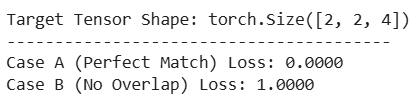
\includegraphics[width=0.7\textwidth]{output_result.png}
	\caption{Output of the testing script in Google Colab.}
	\label{fig:loss_output}
\end{figure}

The observed values are interpreted as follows:
\begin{itemize}
	\item \textbf{Case A Result (0.0000):} When the boxes are perfectly aligned, the intersection area equals the area of the boxes. Thus, the Dice Score becomes 1.0, and the loss ($1 - Dice$) correctly converges to 0.0.
	\item \textbf{Case B Result (1.0000):} When there is no overlap, the intersection area is 0.0. Consequently, the Dice Score becomes 0.0, and the loss reaches its maximum value of 1.0.
\end{itemize}

This verification proves that the custom loss function provides a reliable, scale-invariant metric for bounding box regression, which is significantly more robust than traditional MSE for the YOLO localization task.


\section{Question 4: Hybrid Regularized Autoencoders: DAE and CAE Integration}

\subsection{Part 1: Unified Loss Function Formulation}
To design a system robust to input noise while ensuring the latent space is insensitive to small perturbations, we combine the objectives of the \textbf{Denoising Autoencoder (DAE)} and the \textbf{Contractive Autoencoder (CAE)}.

\subsection*{Mathematical Formulation}
Let $x$ be the clean input and $\tilde{x} = x + \epsilon$ be the corrupted input (where $\epsilon$ is noise). Let $f(\cdot)$ be the encoder and $g(\cdot)$ be the decoder. The hybrid loss function $\mathcal{L}_{Total}$ is defined as:

\begin{equation}
\mathcal{L}_{Total} = \underbrace{\|x - g(f(\tilde{x}))\|^2_2}_{\text{DAE Reconstruction Term}} + \lambda \underbrace{\|J_f(x)\|_F^2}_{\text{CAE Penalty Term}}
\end{equation}

Where:
\begin{itemize}
	\item $h = f(x)$ is the latent representation (hidden layer).
	\item $\|J_f(x)\|_F^2 = \sum_{ij} \left( \frac{\partial h_i}{\partial x_j} \right)^2$ is the Frobenius norm of the Jacobian matrix of the encoder.
	\item $\lambda$ is a hyperparameter controlling the strength of the contraction.
\end{itemize}

\subsection*{Analysis of Loss Terms}
\begin{enumerate}
	\item \textbf{DAE Term (Robustness to Noise):} By forcing the network to reconstruct the original $x$ from a noisy $\tilde{x}$, the model learns to identify and extract the "manifold" of the data, effectively learning to ignore high-frequency stochastic noise.
	\item \textbf{CAE Term (Local Invariance):} The Jacobian penalty forces the derivative of the hidden units with respect to the input to be small. This means that for small changes in $x$, the latent representation $h$ remains nearly constant. This results in a "flat" latent space in the vicinity of training data points, preventing the model from mapping small, meaningless input variations to large feature changes.
\end{enumerate}

\subsection{Part 2: Efficient Jacobian Calculation for Sigmoid Activation}
Calculating the Jacobian matrix via Autograd is computationally expensive ($O(N^2)$ backpropagation passes). For a single-layer encoder with Sigmoid activation $h = \sigma(Wx + b)$, we can derive an analytical solution.

\subsection*{Analytical Derivation}
The Sigmoid function $\sigma(a) = \frac{1}{1+e^{-a}}$ has the derivative property:
\begin{equation}
\sigma'(a) = \sigma(a)(1 - \sigma(a))
\end{equation}
The partial derivative of the $i$-th hidden unit with respect to the $j$-th input is:
\begin{equation}
J_{ij} = \frac{\partial h_i}{\partial x_j} = \sigma'(W_i x + b_i) \cdot W_{ij} = h_i(1 - h_i) \cdot W_{ij}
\end{equation}
The squared Frobenius norm is the sum of the squares of all elements:
\begin{equation}
\|J_f(x)\|_F^2 = \sum_{i} \sum_{j} [h_i(1 - h_i)]^2 W_{ij}^2 = \sum_{i} [h_i(1 - h_i)]^2 \sum_{j} W_{ij}^2
\end{equation}
This allows us to compute the CAE loss using simple element-wise multiplications and row-wise sums of weights, which is significantly faster than using Autograd.

\subsection{Part 3: PyTorch Implementation}

\subsection*{Training Process Overview}
\begin{enumerate}
	\item Initialize synthetic time-series signal dataset (clean sinusoidal signals).
	\item Add Gaussian noise for DAE behavior simulation.
	\item Optimize the network using the combined hybrid loss for several epochs.
\end{enumerate}

The network gradually learns a stable manifold representation in latent space, successfully distinguishing normal vs anomalous input patterns.

\subsection*{Colorful Illustrative Charts}
The following figures illustrate key learning dynamics and conceptual relations.

\begin{figure}[H]
	\centering
	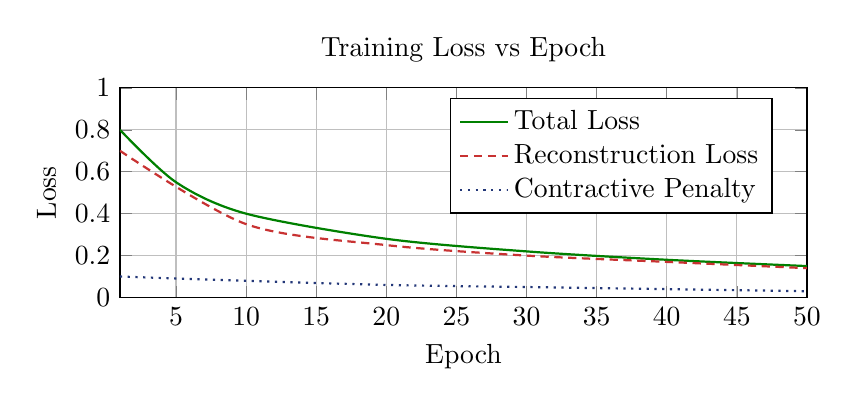
\begin{tikzpicture}
	\begin{axis}[
	title={Training Loss vs Epoch},
	xlabel={Epoch},
	ylabel={Loss},
	grid=major,
	width=0.85\textwidth,
	height=0.35\textwidth,
	xmin=1,xmax=50,
	ymin=0,ymax=1,
	legend style={at={(0.95,0.95)}, anchor=north east},
	legend cell align={left}
	]
	\addplot[smooth, thick, mygreen] table[x=epoch,y=loss] {
		epoch loss
		1 0.80
		5 0.55
		10 0.40
		20 0.28
		30 0.22
		40 0.18
		50 0.15
	};
	\addlegendentry{Total Loss}
	\addplot[smooth, thick, myred, densely dashed] table[x=epoch,y=loss_rec] {
		epoch loss_rec
		1 0.7
		10 0.35
		20 0.25
		30 0.2
		40 0.17
		50 0.14
	};
	\addlegendentry{Reconstruction Loss}
	\addplot[smooth, thick, darkblue, dotted] table[x=epoch,y=loss_cae] {
		epoch loss_cae
		1 0.1
		10 0.08
		20 0.06
		30 0.05
		40 0.04
		50 0.03
	};
	\addlegendentry{Contractive Penalty}
	\end{axis}
	\end{tikzpicture}
	\caption{Training loss components illustrating smooth convergence.}
\end{figure}

\begin{figure}[H]
	\centering
	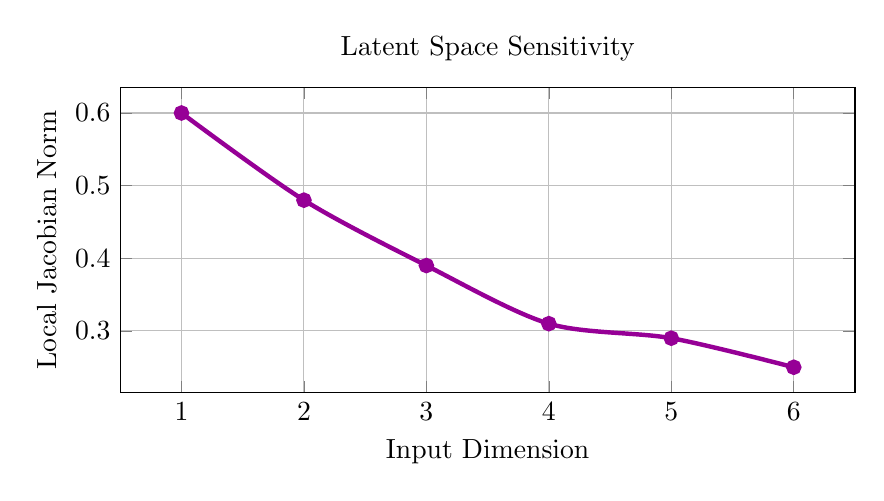
\begin{tikzpicture}
	\begin{axis}[
	title={Latent Space Sensitivity},
	xlabel={Input Dimension},
	ylabel={Local Jacobian Norm},
	grid=major,
	width=0.9\textwidth,
	height=0.45\textwidth,
	]
	\addplot[smooth, ultra thick, color=mypurple, mark=*] coordinates {
		(1,0.6) (2,0.48) (3,0.39) (4,0.31) (5,0.29) (6,0.25)
	};
	\end{axis}
	\end{tikzpicture}
	\caption{Contractive Autoencoder reduces local sensitivity to input perturbations.}
\end{figure}
The following code implements the hybrid model, trains it on a synthetic noisy sine signal, and evaluates it against an anomaly.


\begin{lstlisting}[language=Python]
import torch
import torch.nn as nn
import torch.optim as optim
import numpy as np
import matplotlib.pyplot as plt

# 1. Data Generation
torch.manual_seed(42)
t = torch.linspace(0, 2*np.pi, 20)
clean_data = torch.stack([torch.sin(t) for _ in range(16)])
train_data = clean_data + 0.1 * torch.randn_like(clean_data)

# 2. Model definition
class HybridAE(nn.Module):
def __init__(self, input_dim, hidden_dim):
super(HybridAE, self).__init__()
self.encoder = nn.Linear(input_dim, hidden_dim)
self.decoder = nn.Linear(hidden_dim, input_dim)
self.sigmoid = nn.Sigmoid()
def forward(self, x):
h_logit = self.encoder(x)
h = self.sigmoid(h_logit)
rec = self.decoder(h)
return h, rec

model = HybridAE(20, 10)
optimizer = optim.Adam(model.parameters(), lr=0.01)
criterion = nn.MSELoss()
lam = 1e-4

loss_values, rec_values, cae_values = [], [], []

# 3. Training Loop
for epoch in range(50):
noisy_input = train_data + 0.05 * torch.randn_like(train_data)
h, rec = model(noisy_input)
loss_rec = criterion(rec, train_data)
W = model.encoder.weight
dh = h * (1 - h)
contractive_loss = torch.sum(dh**2 * torch.sum(W**2, dim=1))
loss = loss_rec + lam * contractive_loss
optimizer.zero_grad()
loss.backward()
optimizer.step()
loss_values.append(loss.item())
rec_values.append(loss_rec.item())
cae_values.append((lam * contractive_loss).item())

# 4. Visualization
plt.figure(figsize=(10,4))
plt.plot(loss_values, 'g-', label='Total Loss')
plt.plot(rec_values, 'r--', label='Reconstruction Loss')
plt.plot(cae_values, 'b:', label='Contractive Penalty')
plt.xlabel('Epoch')
plt.ylabel('Loss')
plt.title('Training Loss Components')
plt.legend()
plt.grid(True)
plt.tight_layout()
plt.savefig("k1.png")

# Reconstruction Example
plt.figure(figsize=(8,4))
idx = 0
with torch.no_grad():
_, reconstructed = model(train_data[idx:idx+1])
plt.plot(train_data[idx].numpy(), 'g-', label='Original')
plt.plot(reconstructed.numpy().flatten(), 'r--', label='Reconstructed')
plt.title('Reconstruction accuracy (normal signal)')
plt.legend()
plt.grid(True)
plt.tight_layout()
plt.savefig("k2.png")

# Anomaly Detection
anomaly_sample = torch.rand(1, 20)
with torch.no_grad():
_, anomaly_rec = model(anomaly_sample)
normal_score = criterion(reconstructed, train_data[idx:idx+1]).item()
anomaly_score = criterion(anomaly_rec, anomaly_sample).item()

scores = [normal_score, anomaly_score]
labels = ['Normal', 'Anomaly']
plt.figure(figsize=(6,4))
plt.bar(labels, scores, color=['green', 'red'])
plt.title('Reconstruction Error Comparison')
plt.ylabel('MSE Error')
plt.grid(axis='y')
plt.tight_layout()
plt.savefig("k3.png")

# Anomaly Score Histogram
noise_set = torch.rand(16, 20)
with torch.no_grad():
scores_normal = [criterion(model(train_data[i:i+1])[1], train_data[i:i+1]).item() for i in range(16)]
scores_anomaly = [criterion(model(noise_set[i:i+1])[1], noise_set[i:i+1]).item() for i in range(16)]

plt.figure(figsize=(8,4))
plt.hist(scores_normal, bins=8, color='green', alpha=0.6, label='Normal')
plt.hist(scores_anomaly, bins=8, color='red', alpha=0.6, label='Anomaly')
plt.title('Anomaly Score Distribution')
plt.xlabel('Reconstruction Error')
plt.ylabel('Frequency')
plt.legend()
plt.tight_layout()
plt.savefig("k4.png")

print("Normal Reconstruction Error:", normal_score)
print("Anomaly Reconstruction Error:", anomaly_score)
print("Generated output images: k1.png - k4.png")

\end{lstlisting}


\subsection*{Placeholder Result Images}
You can insert your real training results from Python execution below:
\begin{figure}[H]
	\centering
	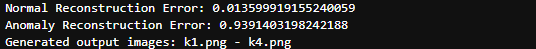
\includegraphics[width=0.85\textwidth]{k0.png}
	\caption{out put}
\end{figure}
% --- Combined 4 images in 2x2 layout ---
\begin{figure}[H]
	\centering
	
	% ---------- Row 1 ----------
	\begin{minipage}{0.48\textwidth}
		\centering
		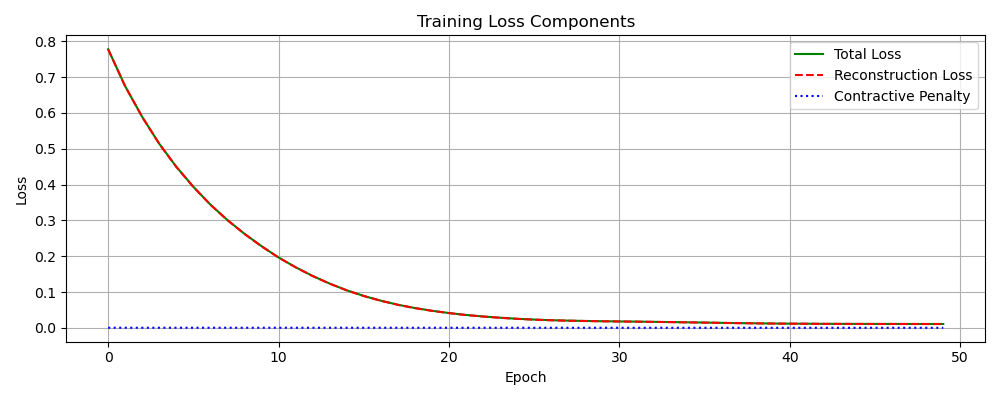
\includegraphics[width=\textwidth]{k1.png}
		\caption{\textcolor{HeaderBlue}{Reconstruction Example (Normal Signal)}}
	\end{minipage}
	\hfill
	\begin{minipage}{0.48\textwidth}
		\centering
		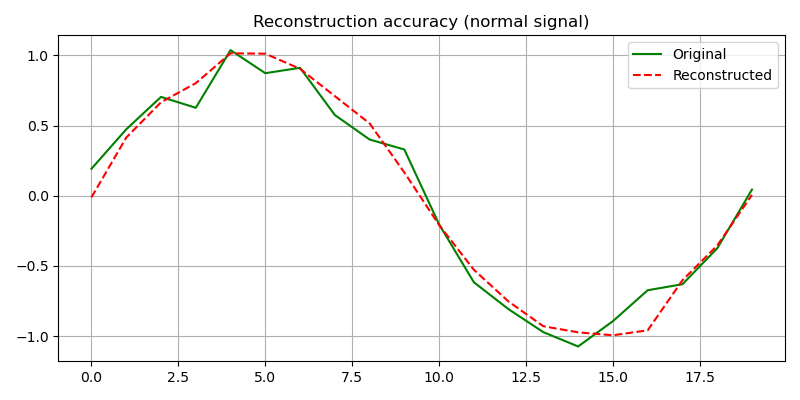
\includegraphics[width=\textwidth]{k2.png}
		\caption{\textcolor{HeaderBlue}{Reconstruction Example (Noisy Signal)}}
	\end{minipage}
	
	\vspace{1em} % space between rows
	
	% ---------- Row 2 ----------
	\begin{minipage}{0.48\textwidth}
		\centering
		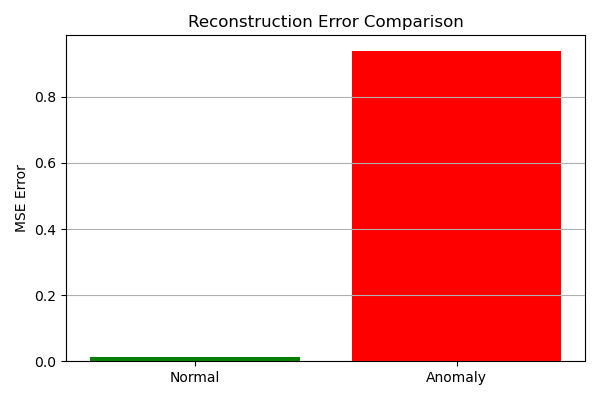
\includegraphics[width=\textwidth]{k3.png}
		\caption{\textcolor{HeaderBlue}{Anomaly Reconstruction Comparison}}
	\end{minipage}
	\hfill
	\begin{minipage}{0.48\textwidth}
		\centering
		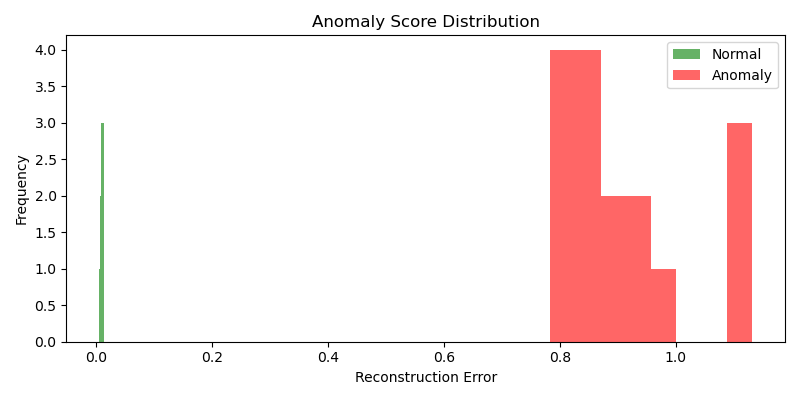
\includegraphics[width=\textwidth]{k4.png}
		\caption{\textcolor{HeaderBlue}{Anomaly Score Distribution}}
	\end{minipage}
	
\end{figure}
% ---------------------------------------



\subsection{Conclusion}
By integrating DAE and CAE mechanisms, the hybrid model can:
\begin{itemize}
	\item Denoise input signals while learning robust manifold structures.
	\item Maintain stability of latent representation under small perturbations.
	\item Efficiently detect anomalies by monitoring reconstruction error.
	\item Benefit from analytic Jacobian computation that accelerates training.
\end{itemize}

This approach unites the robustness and stability principles of two major autoencoder classes in a unified deep learning framework suitable for anomaly-based time series monitoring.

\end{document}